% !TEX root =./main.tex




\begin{abstract}

Sonar, sending and receiving sounds as a sensor, is a valuable tool that electrical and computer engineering provides.  In this project, CPX 3, we are improving upon a provided system.  The system collected data from a phased array of four omni-directional microphones, after a pulse from a single approximately omni-directional speaker.  We are working to improve both the speed and quality of the processing of this data, using the digital signal processing and problem solving techniques learned this semester. [REWRITE THIS ONCE REST IS WRITTEN AND WRITE MORE ABOUT METHODS AND RESULTS]


\end{abstract}

\section{Introduction}

This report presents the design process and outcomes for the development of a sonar system by Three Engineers and Ben Corporation. Leveraging advanced digital signal processing (DSP) techniques and MATLAB design tools, our team implemented an 11-stage sonar processing system. Throughout the project, we faced critical engineering decisions to balance the trade-offs between optimizing the system for high-quality sonar imaging and ensuring fast, real-time display capabilities.

The following sections provide a detailed account of our design approach, implementation, and analysis for each stage of the system. By documenting our decisions and their rationale, this report highlights the innovative solutions and technical expertise that distinguish our sonar processing system.


Sonar, ultrasound, and radar are all based on the same principle: transmit a wave, and record its echos.  The only differences are the type of wave or the frequencies involved.  In this project, we are using sonar.  Working in the audible range enables the use of low-cost, common speakers and microphones.  Additionally, it allows us to hear to pulses and echos, which can serve as another problem solving tool.

For this project, we are working with recorded data.  The recorded data was produced using a single omni-directional speaker to transmit the pulse and a phased array of four omni-directional microphones to receive the echos.  Each microphone is given a channelL $X_1$, $X_2$, $X_3$, and $X_4$.

The signal processing is done inside of a \textsc{Matlab} script, following the process diagrammed in Figure \ref{fig:stages}. 

\begin{figure}[H]
    \centering
    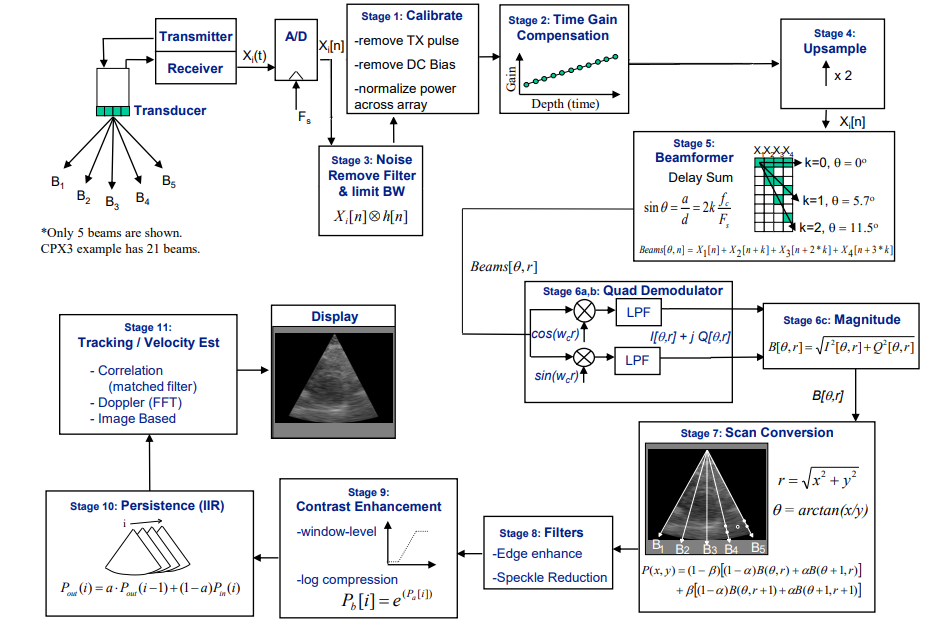
\includegraphics[width=0.75\linewidth]{figures/stages.png}
    \caption{Signal Processing Stages}
    \label{fig:stages}
\end{figure}
